\documentclass[]{beamer}


%%%%%%%%%%%%%%%%%%%%%%%%%%%%% BEAMER SETUP %%%%%%%%%%%%%%%%%%%%%%%%%%%%%%%%%%%%


\usetheme{Warsaw}
\beamertemplatenavigationsymbolsempty

\title[Analysing Handwritten Records]{No Pain, No Gain: The Challenges and Rewards of Analysing Handwritten Records}
\author[Antriksh Dhand]{\texorpdfstring{\textbf{Antriksh Dhand}\\{\small Supervised by Dr.~Jenkin \& Professor Keay}}{\textbf{Antriksh Dhand}}}
\date{May 17th, 2024}

\institute[USYD]
{
	School of Medical Science\\
	The University of Sydney
}

\AtBeginSection[]
{
  \begin{frame}
    \frametitle{Table of Contents}
    \tableofcontents[currentsection]
  \end{frame}
}

%%%%%%%%%%%%%%%%%%%%%%%%%%%%%%%% PACKAGES %%%%%%%%%%%%%%%%%%%%%%%%%%%%%%%%%%%%%

\usepackage{hyperref}

\usepackage{tikz}
\usetikzlibrary{intersections, shapes.geometric, arrows.meta, positioning}

\usepackage{listings}
\usepackage{xcolor}

\usepackage{booktabs}

\usepackage{graphicx} % PDF

\usepackage{animate} % GIF

%%% CODE INPUT %%%
\definecolor{backcolour}{rgb}{0.95,0.95,0.92}
\definecolor{codegray}{rgb}{0.5,0.5,0.5}
\definecolor{backgray}{RGB}{235, 235, 235}

% Code input styling
\lstset{
    language=Python,
    basicstyle=\ttfamily\small,
    numbers=left,
    numberstyle=\tiny\color{codegray},
    columns=fullflexible,
    breaklines=true,
    backgroundcolor=\color{backcolour},
    frame=single,
    showstringspaces=false,
	commentstyle=\color{codegray},
    literate={~} {$\sim$}{1},
	upquote=true
}

% Code output styling
\lstdefinestyle{output}{
    basicstyle=\ttfamily\small,
    backgroundcolor=,
    numbers=none,
    frame=none,
    breaklines=true,
}

%%%%%%%%%%%%%%%%%%%%%%%%%%%%%%%%%%%%%%%%%%%%%%%%%%%%%%%%%%%%%%%%%%%%%%%%%%%%%%%%%

\begin{document}

%%%%%%%%%%%%%%%%%%%%%%%%%
	\begin{frame}
	\titlepage
	\end{frame}
%%%%%%%%%%%%%%%%%%%%%%%%%

%%%%%%%%%%%%%%%%%%%%%%%%%
	\begin{frame}{Table of Contents}
	\tableofcontents
	\end{frame}
%%%%%%%%%%%%%%%%%%%%%%%%%

	\section{Introduction}

	\subsection{Motivation} % Why analyse historical data?

%%%%%%%%%%%%%%%%%%%%%%%%%
\begin{frame}{Why analyse historical records?}
	\begin{columns}
		\begin{column}{0.6\textwidth}
			\begin{itemize}
				\item Importance of preserving history: preventing historical data from decaying unutilised.
				\item Learning about societal trends in the past through their records.
				\item Applying learnings from the past to modern society.
			\end{itemize}
			\vspace{1em}
			See: Hildebrandt (2016), Garton (1988)
		\end{column}
		\begin{column}{0.4\textwidth}
			\begin{figure}
				\includegraphics[width=0.85\textwidth]{img/anatomy_of_murder.jpeg}
			\end{figure}	
		\end{column}
	\end{columns}
\end{frame}
%%%%%%%%%%%%%%%%%%%%%%%%%

%%%%%%%%%%%%%%%%%%%%%%%%%
% \begin{frame}{Why analyse historical records?}
% 	Petrakis et al. reflect on the importance of digitising ship logbooks of the 19\textsuperscript{th} and 20\textsuperscript{th} century:
% 	\begin{itemize}
% 		\item Helps them analyse the transition from sail to steam navigation in the Mediterranean
% 		\begin{itemize}
% 			\item Change in trade routes
% 			\item Changes in duration of voyage
% 			\item Steam ships having to stay shore longer than sail boats due to repairs and servicing
% 		\end{itemize}
% 		\item Local cultural and political factors
% 		\item Uncover details about the working and living conditions and social relations on board

% 		\vspace{0.5em}
% 			\small
% 			\begin{quote}
% 				``In the margin of the logbook [the captain] wrote twice about his disappointment and frustration...reflecting the anxiety and psychological strain on some people working at sea."
% 			\end{quote}
% 	\end{itemize}
% \end{frame}
%%%%%%%%%%%%%%%%%%%%%%%%%

% %%%%%%%%%%%%%%%%%%%%%%%%%
% \begin{frame}{The process of analysing historical registers}

% 	Analysing registers or logbooks is a difficult yet incredibly important task for historical research.\footnotemark
	
% 	\vspace{1em}

% 	The process can largely be separated into three activities:\footnotemark
% 	\begin{enumerate}
% 		\item Data digitisation
% 		\item Data curation
% 		\item Data exploration
% 	\end{enumerate}

% 	\footnotetext{Oliver, J. and Kington, J.A. (1970)}
% 	\footnotetext{Petrakis, K. et al. (2021)}
% \end{frame}
% %%%%%%%%%%%%%%%%%%%%%%%%%

	\subsection{Background}

%%%%%%%%%%%%%%%%%%%%%%%%%
\begin{frame}[fragile]{Introduction to the Anatomy Registers project}
	\begin{figure}
		\includegraphics[height=0.7\textheight]{img/register/serious_cursive.png}
		\caption{The primary data in this research project: the Anatomy Registers}
	\end{figure}
\end{frame}
%%%%%%%%%%%%%%%%%%%%%%%%%

%%%%%%%%%%%%%%%%%%%%%%%%%
\begin{frame}[fragile]{Introduction to the dataset}
	13 attributes taken from the anatomy registers:

	\begin{columns}[T]
		\begin{column}{0.5\textwidth}
			\begin{itemize}
				\item Year
				\item ID
				\item Sex
				\item Age
				\item Cause of death
				\item Place of death
				\item Time of reception
			\end{itemize}
		\end{column}
		\begin{column}{0.5\textwidth}
			\begin{itemize}
				\item Date of death
				\item Date of reception
				\item Date of return for sepulture
				\item Date of burial or cremation
				\item Retention time
				\item Cemetery
			\end{itemize}	
		\end{column}
	\end{columns}
\end{frame}
%%%%%%%%%%%%%%%%%%%%%%%%%

%%%%%%%%%%%%%%%%%%%%%%%%%
\begin{frame}[fragile]{Introduction to the Anatomy Registers project}
	\begin{figure}
		\includegraphics[width=\textwidth]{img/excel_dataset.png}
		\caption{From cursive to Calibri -- the first few rows of Dr.~Jenkin's transcribed data}
	\end{figure}
\end{frame}
%%%%%%%%%%%%%%%%%%%%%%%%%

%%%%%%%%%%%%%%%%%%%%%%%%%
\begin{frame}[fragile]{Introduction to the dataset}

	\begin{itemize}
		\item The dataset contained 7609 records spanning 101 years from 1883 to 1983.
		\item The format was typical of most manually-collected datasets.
		\item No cleaning had been conducted on the dataset, other than basic checks during entry.
		\item All data was de-identified in line with USYD's Human Research Ethics Committee approval.\footnotemark
	\end{itemize}

	\footnotetext{\textit{``Investigation of historical, demographic and medical information in cadaver records held by the Discipline of Anatomy."} Project 2017/898}

\end{frame}
%%%%%%%%%%%%%%%%%%%%%%%%%

% %%%%%%%%%%%%%%%%%%%%%%%%%
% \begin{frame}[fragile, plain]{Introduction to the dataset}
% 	\framesubtitle{Preliminary data analysis}

% 	\centering
% 	\begin{figure}
% 		\includegraphics[width=\textwidth]{img/data_by_year.pdf}
% 	\end{figure}	
% 	% Insert chart of number of entries per year

% \end{frame}
% %%%%%%%%%%%%%%%%%%%%%%%%%

% %%%%%%%%%%%%%%%%%%%%%%%%%
% \begin{frame}[fragile, plain]{Introduction to the dataset}
% 	\framesubtitle{Preliminary data analysis}

% 	% Men vs Women
% 	\centering
% 	\begin{figure}
% 		\includegraphics[width=\textwidth]{img/data_by_sex.pdf}
% 	\end{figure}	

% \end{frame}
% %%%%%%%%%%%%%%%%%%%%%%%%%

	\subsection{Project scope}

%%%%%%%%%%%%%%%%%%%%%%%%%
\begin{frame}{The scope for SCDL3991}
		% This was my first time working with first-hand historical data 
		% At uni, data is polished by coordinators before setting it for analysis

	\begin{alertblock}{Original project aim}
		Compare cause of death with place of death to uncover trends in regards to how and where people died.
	\end{alertblock}

	\begin{exampleblock}{Updated project aim}
		Improve the data quality of the Asset Register dataset and bring it into a state useable for analysis.
	\end{exampleblock}

	\vspace{1em}
	% This was our aim \textit{under the assumption that the data would be in a programmatically useable state.}

\end{frame}
%%%%%%%%%%%%%%%%%%%%%%%%%


% %%%%%%%%%%%%%%%%%%%%%%%%%
% \begin{frame}{The scope for SCDL3991}

% 	{\large \textbf{This project is the product of discovering that historical data -- especially hand-transcribed data -- is rarely ready for analysis out of the box.}}

% 	\vspace{1em}

% 	\onslide{Why?}
% 	\begin{itemize}
% 		\item<2-> Records are usually transcribed in the pursuit of retaining history, not necessarily for the purposes of analysis. % Talk about people coming to the Anatomy records to find information about their ancestor.
% 		\item<3-> The process of digitising old records written in cursive script is incredibly laborious and error-prone.
% 	\end{itemize}
% 	% As a result, our project aim shifted.

% \end{frame}
% %%%%%%%%%%%%%%%%%%%%%%%%%


% %%%%%%%%%%%%%%%%%%%%%%%%%
% \begin{frame}{The scope for SCDL3991}

% 	\begin{exampleblock}{Updated project aim}
% 		Improve the data quality of the Asset Register dataset and bring it into a state useable for analysis.
% 	\end{exampleblock}

% 	\vspace{1em}

% 	We will demonstrate our success by performing a geographical analysis on the ``place of death" attribute.

% \end{frame}
% %%%%%%%%%%%%%%%%%%%%%%%%%

	\section{Methodology: The Pain}

% %%%%%%%%%%%%%%%%%%%%%%%%%
% \begin{frame}{A note on exclusivity}

% 	\begin{itemize}
% 		\item The following section will present some data quality issues found in the Anatomy Registers dataset.
% 		\item The data quality issues which will be presented in this section are \textbf{not unique to this project alone.}
% 		\item Consequently, the solutions we will discuss are broadly applicable and not restricted solely to this dataset.
% 	\end{itemize}
% \end{frame}
% %%%%%%%%%%%%%%%%%%%%%%%%%

	\subsection{Data verification and validation}

%%%%%%%%%%%%%%%%%%%%%%%%%
\begin{frame}[fragile]{Ensuring data completeness}
	\begin{block}{Data completeness}
		The extent to which all required or expected records and data fields are present in a dataset.
	\end{block}
	\vspace{1em}
	Potential solutions:
	\begin{itemize}
		\item Delete the missing entry
		\item Replace with a statistical summary (mean/median)
		\item Impute the missing value based on context
	\end{itemize}
\end{frame}
%%%%%%%%%%%%%%%%%%%%%%%%%

%%%%%%%%%%%%%%%%%%%%%%%%%
\begin{frame}[fragile]{Ensuring data completeness}

	\begin{lstlisting}
data.isna().sum()
	\end{lstlisting}

	\begin{columns}
		\column{0.6\textwidth}
			\begin{lstlisting}[style=output]
year                        0
id                          0
sex                         5
age                        10
death_date               2436
reception_date              0
return_date_sepulture    1680
burial_date              4408
death_place                 6
place_code                  0
			\end{lstlisting}
		\column{0.3\textwidth}
		\begin{exampleblock}{Solution}
			Replaced missing date of death with the date the body reached USYD
		\end{exampleblock}
	\end{columns}
\end{frame}
%%%%%%%%%%%%%%%%%%%%%%%%%

%%%%%%%%%%%%%%%%%%%%%%%%%
\begin{frame}[fragile]{Ensuring data consistency}

	\begin{block}{Data consistency}
		Data adheres to a set of predefined rules and formats, ensuring uniformity in the representation of information.
	\end{block}
	i.e. The representation of the data is actually useable (programmatically or in the dataset itself).

\end{frame}
%%%%%%%%%%%%%%%%%%%%%%%%%

%%%%%%%%%%%%%%%%%%%%%%%%%
\begin{frame}[fragile]{Ensuring data consistency}
	\framesubtitle{Formatting dates correctly}

	Check to see if our 4 date columns are in the right format: \texttt{death\_date}, \texttt{reception\_date}, \texttt{return\_date\_sepulture} and \texttt{burial\_date}.

	\begin{figure}[width=\textwidth]
		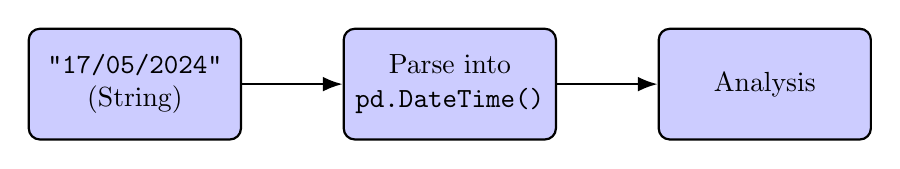
\begin{tikzpicture}[node distance=4cm, auto, thick]

			% Define style for boxes
			\tikzstyle{block} = [rectangle, draw, fill=blue!20, 
								text width=7em, text centered, 
								rounded corners, minimum height=4em]
		
			% Define style for arrows
			\tikzstyle{line} = [draw, -{Latex[length=2.5mm]}]
		
			% Place nodes
			\node [block] (init) {\texttt{"17/05/2024"} (String)};
			\node [block, right of=init] (datetime) {Parse into \texttt{pd.DateTime()}};
			\node [block, right of=datetime] (analysis) {Analysis};
		
			% Draw edges
			\path [line] (init) -- (datetime);
			\path [line] (datetime) -- (analysis);
		\end{tikzpicture}
	\end{figure}

\end{frame}
%%%%%%%%%%%%%%%%%%%%%%%%%

%%%%%%%%%%%%%%%%%%%%%%%%%
\begin{frame}[fragile]{Ensuring data consistency}
	\framesubtitle{Formatting dates correctly}

	\begin{exampleblock}{\small Match dates in the format DD/MM/YYYY}
		\small\texttt{"\textasciicircum(0?[0-9]|[12]\textbackslash d|3[01])\/(0?[0-9]|1[0-2])\/(000\textbackslash d|00\textbackslash d\{2\}\\|0\textbackslash d\{3\}|1\textbackslash d\{3\}|2000)\$"}
	\end{exampleblock}

	\begin{itemize}
		\item \small \textbf{Day Component:} \texttt{"\textasciicircum(0?[0-9]|[12]\textbackslash d|3[01])"}
		\begin{itemize}
		  \item \texttt{"0?[0-9]"}: Matches a single digit day from 01 to 09
		  \item \texttt{"[12]\textbackslash d"}: Matches any two-digit day from 10 to 29
		  \item \texttt{"3[01]"}: Matches the days 30 or 31
		\end{itemize}
	  
		\item \small \textbf{Month Component:} \texttt{"(0?[0-9]|1[0-2])"}
		\begin{itemize}
		  \item \texttt{"0?[0-9]"}: Matches a single digit month from 01 to 09
		  \item \texttt{"1[0-2]"}: Matches the months 10, 11, and 12
		\end{itemize}
	  
		\item \small \textbf{Year Component:} \texttt{"(000\textbackslash d|00\textbackslash d\{2\}|0\textbackslash d\{3\}|1\textbackslash d\{3\}|2000)"}
		\begin{itemize}
		  \item Iteratively matches any year between 0000 and 2000
		\end{itemize}
	\end{itemize}
\end{frame}
%%%%%%%%%%%%%%%%%%%%%%%%%

%%%%%%%%%%%%%%%%%%%%%%%%%
\begin{frame}[fragile]{Ensuring data consistency}
	\framesubtitle{Formatting dates correctly}
	\begin{lstlisting}
data[~data["death_date"].str.match(regex)]
	\end{lstlisting}
	\vspace{1em}
	Some notable findings from running the regex matcher on our dataset:

	\begin{itemize}
		\item \pause \texttt{id=5044, death\_date = "20/11/9161"}
		\item \pause \texttt{id=5014, death\_date = "26/87/1961"}
		\item \pause \texttt{id=5424, death\_date = "31/06/1964"}
	\end{itemize}

\end{frame}
%%%%%%%%%%%%%%%%%%%%%%%%%

%%%%%%%%%%%%%%%%%%%%%%%%%
\begin{frame}[fragile]{Ensuring data validity}

	\begin{block}{Data validity}
		The data accurately represents the real-world values it is supposed to depict.
	\end{block}
	i.e. The values in the dataset make sense. This often involves checking the values of one attribute against another.

\end{frame}
%%%%%%%%%%%%%%%%%%%%%%%%%

%%%%%%%%%%%%%%%%%%%%%%%%%
\begin{frame}[fragile]{Ensuring data validity}
	\framesubtitle{Checking the relationship between dates}

	\begin{lstlisting}
# Entries with difference greater than 10 days
data[(data["reception_date"] - data["death_date"]).dt.days > 10]

# Entries where death_date is after reception_date
data[data["death_date"] > data["reception_date"]]

	\end{lstlisting}

	\begin{table}[]
		\begin{tabular}{lll}
		\toprule
		id   & death\_date & reception\_date \\ \midrule
		1560 & 26/03/1913  & 27/03/1916      \\
		5036 & 23/10/1961  & 23/10/1951		 \\
		\bottomrule
		\end{tabular}
	\end{table}
	In reality, there were dozens of such entries.	
\end{frame}
%%%%%%%%%%%%%%%%%%%%%%%%%

	\subsection{Data transformation}

%%%%%%%%%%%%%%%%%%%%%%%%%
\begin{frame}{Introduction to data transformation}
	
	Data transformation involves transforming some parts of the dataset in order to make performing statistical analysis on it more feasible.\\
	\vspace{1em}	
	Often, unstructured data (such as textual data) benefits the most from such data cleaning.
\end{frame}
%%%%%%%%%%%%%%%%%%%%%%%%%

% %%%%%%%%%%%%%%%%%%%%%%%%%
% \begin{frame}{Why handwritten data can be so unstructured}
	
%     \begin{block}{\textit{Anatomy Act (1881)}}
%         \begin{quote}\small{Every person so receiving a body for anatomical examination...shall demand and receive together with the body...a return stating at what day and hour and from whom the body was received, the date and \alert{place of death}, the sex, and (as far as is known at the time) the Christian and surname, age and last place of abode of such person...}\end{quote}
%     \end{block}
% 	\vspace{1em}
% 	The level of detail and structure of the entry was completely up to the practitioner.
% \end{frame}
% %%%%%%%%%%%%%%%%%%%%%%%%%

%%%%%%%%%%%%%%%%%%%%%%%%%
\begin{frame}[fragile]{A range of responses in \texttt{death\_place}}

	Some practitioners took extreme care and precision when entering in the place of death:
	\begin{itemize}
		\item \small ``Former" and ``new" names
		\begin{itemize}
			\item \texttt{st george district hospital \alert{formerly} 301 queen st concord west}
			\item \texttt{netherleigh private hospital \alert{now} eastern suburbs private hospital chapel st randwick}
		\end{itemize}

		\item \small Compound locations
		\begin{itemize}
			\item \texttt{hornsby hospital \alert{from} oatlands nursing home dundas}
			\item \texttt{9 redmyre rd strathfield \alert{and} royal north shore hospital}
		\end{itemize}
	\end{itemize}

\end{frame}
%%%%%%%%%%%%%%%%%%%%%%%%%

%%%%%%%%%%%%%%%%%%%%%%%%%
\begin{frame}[fragile]{A range of responses in \texttt{death\_place}}

	Some practioners were on the other end of detail:
	\begin{itemize}
		\item \small Minimally descriptive entries 
		\begin{itemize}
			\item \texttt{at home}
			\item \texttt{donor}
			\item \texttt{morgue}
		\end{itemize}
		\item \small Suburbs only
		\begin{itemize}
			\item \texttt{orange}
			\item \texttt{waverley}
		\end{itemize}
	\end{itemize}

\end{frame}
%%%%%%%%%%%%%%%%%%%%%%%%%

%%%%%%%%%%%%%%%%%%%%%%%%%
\begin{frame}[fragile]{A range of responses in \texttt{death\_place}}

	And some practioners were in-between:
	\begin{itemize}
		\item \texttt{royal prince alfred hospital camperdown page pavilion}
		\item \texttt{royal prince alfred hospital}
		\item \texttt{rpa}
	\end{itemize}

\end{frame}
%%%%%%%%%%%%%%%%%%%%%%%%%

%%%%%%%%%%%%%%%%%%%%%%%%%
\begin{frame}[fragile]{A range of responses in \texttt{death\_place}}

	Some people passed away in odd spots:
	\begin{itemize}
		\item \texttt{in omnibus kingslangly rd greenwich}
		\item \texttt{at sea ss ellinis}
		\item \texttt{in the road guildford rd guildford}
	\end{itemize}

\end{frame}
%%%%%%%%%%%%%%%%%%%%%%%%%

%%%%%%%%%%%%%%%%%%%%%%%%%
\begin{frame}[fragile, plain]{}

	% Background with text strings, repeated and scattered
    \begin{tikzpicture}[remember picture, overlay]
        \node[text opacity=0.05, scale=1.0, text width=1.4\paperwidth] at (current page.center) {
            \huge\texttt{
            st george district hospital formerly 301 queen st concord west netherleigh private hospital now eastern suburbs private hospital chapel st randwick hornsby hospital from oatlands nursing home dundas \\
            9 redmyre rd strathfield and royal north shore hospital at home donor morgue orange waverley royal prince alfred hospital camperdown page pavilion royal prince alfred hospital rpa in omnibus kinslangly rd greenwich at sea ss ellinis in the road guildford rd guildford st george district hospital formerly 
            st george district hospital formerly 301 queen st concord west netherleigh private hospital now eastern suburbs private hospital chapel st randwick hornsby hospital from oatlands nursing home dundas 9 redmyre rd strathfield and royal north shore hospital at home donor morgue orange waverley royal prince alfred hospital camperdown page pavilion royal prince alfred hospital rpa in omnibus kinslangly rd greenwich \\
            at sea ss ellinis in the road guildford rd guildford \\
            st george district hospital formerly
            }
        };
    \end{tikzpicture}

	\vfill

	% Central question
	\begin{center}
		\Huge Where do you even begin to analyse such varied data?
	\end{center}

	\vfill

\end{frame}
%%%%%%%%%%%%%%%%%%%%%%%%%

%%%%%%%%%%%%%%%%%%%%%%%%%
\begin{frame}{Categorisation of \texttt{death\_place} institution}
		\begin{table}[h]
			\centering
			\resizebox{\textwidth}{!}{
				\begin{tabular}{ll}
					\toprule
					\textbf{Category} & \textbf{Classification criteria} \\
					\midrule
					Private residence & A private address (commencing with a street, flat, lot or unit number) \\
					Aged care & Locations containing ``Nursing", ``Convalescent", ``Aged Care", \ldots \\
					Hospice & Locations containing ``Hospice" + some known hospices \\
					Private hospital & Locations containing ``Private Hospital" or ``surgery" \\
					Public hospital & All hospitals without ``private" in their name, including district hospitals \\
					Public asylum & Currently coded 12 + three special cases (Liverpool, George St, Rockwood) \\
					Public mental asylum & Currently coded 13 + locations containing ``mental asylum" or ``psychiatric" \\
					Aged 2 and under & Currently coded 70 \\
					Morgues & Currently coded 6 + locations containing ``morgue" \\
					Other & Other \\
					\bottomrule
				\end{tabular}
			}
		\end{table}

\end{frame}
%%%%%%%%%%%%%%%%%%%%%%%%%

% %%%%%%%%%%%%%%%%%%%%%%%%%
% \begin{frame}[fragile]{Categorisation of \texttt{death\_place} institution}

% 	Used regular expressions and keyword analysis to extract $\sim$7000 entries into 9 categories.
% 	\vspace{0.5em}
% 	\begin{lstlisting}
% # Example of extracting private residences
% address_keywords = ["avenue", "av", "ave", ...]
% address_pattern = fr"^\d.*\b(?:{'|'.join(address_keywords)})\b"
% 	\end{lstlisting}
% 	\begin{itemize}
% 		\item The above regex expression will classify any entry beginning with a number followed by at least one address keyword as a ``private residence"
% 	\end{itemize}

% \end{frame}
% %%%%%%%%%%%%%%%%%%%%%%%%%

%%%%%%%%%%%%%%%%%%%%%%%%%
\begin{frame}[fragile]{Extracting suburbs from \texttt{death\_place}}
	Another transformation we could perform using the place of death attribute is to categorise it based on the suburb of where the patient died.

	\begin{figure}
		\includegraphics[width=\textwidth]{img/suburb_categorisation.png}
	\end{figure}
\end{frame}
%%%%%%%%%%%%%%%%%%%%%%%%%

%%%%%%%%%%%%%%%%%%%%%%%%%
\begin{frame}[fragile]{Extracting suburbs from \texttt{death\_place}}
	We utilised a NSW Government dataset containing the geographical boundaries of all localities in New South Wales.	
	\vspace{1em}
	\begin{table}[]
		\begin{tabular}{@{}ll@{}}
		\toprule
		suburb      & geometry      \\ \midrule
		Aarons Pass & \texttt{POLYGON (...)} \\
		Abbotsbury  & \texttt{POLYGON (...)} \\
		Abbotsford  & \texttt{POLYGON (...)} \\
		Abercrombie & \texttt{POLYGON (...)} \\ 
		Abercrombie River & \texttt{POLYGON (...)} \\
		\ldots & \ldots \\ \bottomrule
		\end{tabular}
	\end{table}

\end{frame}
%%%%%%%%%%%%%%%%%%%%%%%%%

%%%%%%%%%%%%%%%%%%%%%%%%%
\begin{frame}[fragile]{Extracting suburbs from \texttt{death\_place}}
	\begin{lstlisting}
regex = r'\b(' + '|'.join(suburbs) + r')\b'
matches = donors["death_place"].str.extractall(regex)
	\end{lstlisting}

	Some entries were matched with multiple suburbs.

	\begin{table}[]
		\small
		\begin{tabular}{@{}llll@{}}
		\toprule
		id   & suburb\_1   & suburb\_2 & suburb\_3 \\ \midrule
		\ldots & \ldots	   & \ldots    & \ldots    \\
		7601 & ettrick     & ashbury   & - \\
		7602 & lidcombe    & - & -  \\
		7603 & castle hill & - & - \\
		7604 & rockdale    & woodford  & banksia   \\ \bottomrule
		\end{tabular}
	\end{table}
	e.g. \texttt{"rockdale nursing home 22 woodford st banksia"}
\end{frame}
%%%%%%%%%%%%%%%%%%%%%%%%%

% %%%%%%%%%%%%%%%%%%%%%%%%%
% \begin{frame}[fragile]{Extracting suburbs from \texttt{death\_place}}

% 	\begin{center}
% 		{\large \texttt{"rockdale nursing home 22 woodford st banksia"}}
% 	\end{center}
		
% 	\vspace{2em}

% 	Cleaned these through:
% 	\begin{itemize}
% 		\item Taking the last suburb in the entry (due to structure of addresses)
% 		\item Manually entering for $\sim$100 entries
% 	\end{itemize}
% \end{frame}
% %%%%%%%%%%%%%%%%%%%%%%%%%

	\section{Results: The Gain}

	\subsection{A geographical analysis of donor data}

%%%%%%%%%%%%%%%%%%%%%%%%%
\begin{frame}[plain]{A Geographical Analysis of Donor Data}
	\begin{figure}
		\includegraphics[width=\textwidth]{img/choropleth_counts.png}
		\vspace{-1.5em}
		\caption{A visual guide to donor contributions across NSW suburbs}
	\end{figure}
\end{frame}
%%%%%%%%%%%%%%%%%%%%%%%%%

% %%%%%%%%%%%%%%%%%%%%%%%%%
% \begin{frame}[plain]{A Geographical Analysis of Donor Data}
% 	\begin{figure}
% 		\includegraphics[width=0.92\textwidth]{img/choropleth_category.png}
% 		\vspace{-0.5em}
% 		\caption{The spread of place of death categories across NSW}
% 	\end{figure}
% \end{frame}
% %%%%%%%%%%%%%%%%%%%%%%%%%

%%%%%%%%%%%%%%%%%%%%%%%%%
\begin{frame}[fragile, plain]{A Geographical Analysis of Donor Data}
	\begin{figure}
		\includegraphics[width=0.92\textwidth]{img/choropleth_time/choropleth-1.png}
	\end{figure}
\end{frame}
%%%%%%%%%%%%%%%%%%%%%%%%%

%%%%%%%%%%%%%%%%%%%%%%%%%
\begin{frame}[fragile, plain]{A Geographical Analysis of Donor Data}
	\begin{figure}
		\includegraphics[width=0.92\textwidth]{img/choropleth_time/choropleth-2.png}
	\end{figure}
\end{frame}
%%%%%%%%%%%%%%%%%%%%%%%%%


%%%%%%%%%%%%%%%%%%%%%%%%%
\begin{frame}[fragile, plain]{A Geographical Analysis of Donor Data}
	\begin{figure}
		\includegraphics[width=0.92\textwidth]{img/choropleth_time/choropleth-3.png}
	\end{figure}
\end{frame}
%%%%%%%%%%%%%%%%%%%%%%%%%


%%%%%%%%%%%%%%%%%%%%%%%%%
\begin{frame}[fragile, plain]{A Geographical Analysis of Donor Data}
	\begin{figure}
		\includegraphics[width=0.92\textwidth]{img/choropleth_time/choropleth-4.png}
	\end{figure}
\end{frame}
%%%%%%%%%%%%%%%%%%%%%%%%%


%%%%%%%%%%%%%%%%%%%%%%%%%
\begin{frame}[fragile, plain]{A Geographical Analysis of Donor Data}
	\begin{figure}
		\includegraphics[width=0.92\textwidth]{img/choropleth_time/choropleth-5.png}
	\end{figure}
\end{frame}
%%%%%%%%%%%%%%%%%%%%%%%%%


%%%%%%%%%%%%%%%%%%%%%%%%%
\begin{frame}[fragile, plain]{A Geographical Analysis of Donor Data}
	\begin{figure}
		\includegraphics[width=0.92\textwidth]{img/choropleth_time/choropleth-6.png}
	\end{figure}
\end{frame}
%%%%%%%%%%%%%%%%%%%%%%%%%


%%%%%%%%%%%%%%%%%%%%%%%%%
\begin{frame}[fragile, plain]{A Geographical Analysis of Donor Data}
	\begin{figure}
		\includegraphics[width=0.92\textwidth]{img/choropleth_time/choropleth-7.png}
	\end{figure}
\end{frame}
%%%%%%%%%%%%%%%%%%%%%%%%%


%%%%%%%%%%%%%%%%%%%%%%%%%
\begin{frame}[fragile, plain]{A Geographical Analysis of Donor Data}
	\begin{figure}
		\includegraphics[width=0.92\textwidth]{img/choropleth_time/choropleth-8.png}
	\end{figure}
\end{frame}
%%%%%%%%%%%%%%%%%%%%%%%%%


%%%%%%%%%%%%%%%%%%%%%%%%%
\begin{frame}[fragile, plain]{A Geographical Analysis of Donor Data}
	\begin{figure}
		\includegraphics[width=0.92\textwidth]{img/choropleth_time/choropleth-9.png}
	\end{figure}
\end{frame}
%%%%%%%%%%%%%%%%%%%%%%%%%

%%%%%%%%%%%%%%%%%%%%%%%%%
\begin{frame}[fragile, plain]{A Geographical Analysis of Donor Data}
	\begin{figure}
		\includegraphics[width=0.92\textwidth]{img/choropleth_time/choropleth-10.png}
	\end{figure}
\end{frame}
%%%%%%%%%%%%%%%%%%%%%%%%%

%%%%%%%%%%%%%%%%%%%%%%%%%
\begin{frame}[fragile, plain]{A Geographical Analysis of Donor Data}
	\begin{figure}
		\includegraphics[width=0.92\textwidth]{img/choropleth_time/choropleth-11.png}
	\end{figure}
\end{frame}
%%%%%%%%%%%%%%%%%%%%%%%%%

% %%%%%%%%%%%%%%%%%%%%%%%%%
% \begin{frame}{A Geographical Analysis of Donor Data}
% 	\begin{itemize}
% 		\item Until about 1950, almost all donors were exclusively unclaimed bodies from public and mental asylums.
% 		\item In the 1960's there was a huge amount of donors coming from private residences.
% 		\item This reflected society's changing views on becoming a donor for anatomical purposes.
% 	\end{itemize}
% \end{frame}
% %%%%%%%%%%%%%%%%%%%%%%%%%

	\section{Conclusion}

%%%%%%%%%%%%%%%%%%%%%%%%%
\begin{frame}{Conclusion}

	% {\huge Working with hand-transcribed data is difficult.}
	% \vspace{0.75em}
	% \begin{itemize}
	% 	\item \pause You will need to go through a rigorous data V\&V process
	% 	\item \pause You may need to abstract certain attributes of your data due to their unstructured format
	% \end{itemize}

	
	\begin{itemize}
		\item Working with hand-transcribed data poses unique challenges as a data analyst, requiring a rigorous and time-consuming data verification process.
		\item Interesting results can be achieved through structuring data to determine relationships in the dataset.
	\end{itemize}


\end{frame}
%%%%%%%%%%%%%%%%%%%%%%%%%

%%%%%%%%%%%%%%%%%%%%%%%%%
% \begin{frame}{Conclusion}

% 	{\Large But it's worth it in the end.}

% 	\vspace{0.75em}

% 	Records from the past give you an incomparable insight into society's functioning at the time.

% \end{frame}
% %%%%%%%%%%%%%%%%%%%%%%%%%

\subsection{Limitations}

%%%%%%%%%%%%%%%%%%%%%%%%%
\begin{frame}{Limitations}
	The unstructured attributes in the dataset reduces data quality and limits potential statistical analysis that may uncover interesting findings.

	% Correlation and regression
	% Machine learning
	% Buzz words
\end{frame}
%%%%%%%%%%%%%%%%%%%%%%%%%

	\subsection{Future work}

% %%%%%%%%%%%%%%%%%%%%%%%%%
% \begin{frame}{Future work}
% 	% After cleaning hundreds of entries in order to produce a cleaned version of the Anatomy Registers dataset, exploring trends in the place of death attribute was just the start of countless investigations which could unfold using this data.
% \end{frame}
% %%%%%%%%%%%%%%%%%%%%%%%%%

%%%%%%%%%%%%%%%%%%%%%%%%%
\begin{frame}{Future work}
	\framesubtitle{Further standardisation of place of death}
	As a result, it is important to spend more time cleaning and structuring the data and attributes to allow for complex analysis.

	\vspace{1em}

	e.g. How can we programmatically consolidate similar entries into one?

	\begin{figure}
		\includegraphics[width=\textwidth]{img/deduplication2.png}
	\end{figure}	
\end{frame}
%%%%%%%%%%%%%%%%%%%%%%%%%

%%%%%%%%%%%%%%%%%%%%%%%%%
\begin{frame}{Future work}
	\framesubtitle{Further standardisation of place of death}

	We tried to achieve this using:
	\begin{itemize}
		\item String similarity techniques
		\begin{itemize}
			\item Difficult to find the one best similarity cut-off
			\item Either too harsh e.g. won't allow for absence of address
			\item Or too lenient e.g. will group \texttt{balmain district hospital} and \texttt{bowral district hospital} together
		\end{itemize}
		\item Simple ML approaches
		\begin{itemize}
			\item Attempted to use KMeans clustering (unsupervised learning) to try and cluster the entries together
			\item An issue was that we needed to specify the number of clusters, which is unknown
		\end{itemize}
	\end{itemize}

\end{frame}
%%%%%%%%%%%%%%%%%%%%%%%%%

% %%%%%%%%%%%%%%%%%%%%%%%%%
% \begin{frame}{Explore cause of death}

% 	\begin{exampleblock}{}
% 		Could we trace out the birth of new medical fields using this data?
% 	\end{exampleblock}

% 	\begin{itemize}
% 		\item Psychiatry and psychology are relatively new fields in medicine, both emerging to great extent in the 19th and 20th centuries.
% 		\item Could we potentially trace out the emergence or disappearance of certain terminology in medicine, such as those for mental illness, through analysing the cause of death attribute?
% 	\end{itemize}

% \end{frame}
% %%%%%%%%%%%%%%%%%%%%%%%%%

% %%%%%%%%%%%%%%%%%%%%%%%%%
% \begin{frame}[fragile]{Explore cause of death}
% 	\framesubtitle{Using topic modelling}

% 	\begin{figure}
% 		\includegraphics[width=0.9\textwidth]{img/blei.png}
% 		\caption{Figure 3 from Blei's seminal paper (2006) on the field of topic modelling showing the popularity of three topics in physics based off analysing 100 years worth of \textit{Nature} articles.}
% 	\end{figure}

% \end{frame}
% %%%%%%%%%%%%%%%%%%%%%%%%%

	\subsection{Closing}

%%%%%%%%%%%%%%%%%%%%%%%%%
\begin{frame}{Resources}
	\begin{columns}
		\begin{column}{0.7\textwidth}
			All code written for this project is available in a well-documented Jupyter Notebook, which can be accessed at \textcolor{cyan}{\href{https://github.com/antrikshdhand/SCDL3991-research}{github.com/antrikshdhand/SCDL3991-research}}.
		\end{column}
		\begin{column}{0.3\textwidth}
			\centering
			\includegraphics[width=\textwidth]{img/github.png}
		\end{column}
	\end{columns}
\end{frame}
%%%%%%%%%%%%%%%%%%%%%%%%%

%%%%%%%%%%%%%%%%%%%%%%%%%
\begin{frame}{Acknowledgements}
	I extend my deepest appreciation to my supervisors, Dr. Rebekah Jenkin and Professor Kevin Keay, for helping me see this project through from start to finish despite the many roadblocks in the middle. This project would not have been made possible without our extensive, and often tangential, discussions. 
\end{frame}
%%%%%%%%%%%%%%%%%%%%%%%%%

%%%%%%%%%%%%%%%%%%%%%%%%%
	\begin{frame}
		\centering
		\vspace{30pt}
		{\Huge\textbf{Thank You}}\\

		\vspace{30pt}

		{\Large Any questions?}

		\vspace{30pt}

		\large
		\begin{block}{Contact information}
			\begin{itemize}
				\item Email: \textcolor{cyan}{\href{mailto:adha5655@uni.sydney.edu.au}{adha5655@uni.sydney.edu.au}}
				\item GitHub: \textcolor{cyan}{\href{https://github.com/antrikshdhand}{github.com/antrikshdhand}}
				\item LinkedIn: \textcolor{cyan}{\href{https://www.linkedin.com/in/antrikshdhand}{linkedin.com/in/antrikshdhand}}
			\end{itemize}
	\end{block}
	\end{frame}
%%%%%%%%%%%%%%%%%%%%%%%%%

%%%%%%%%%%%%%%%%%%%%%%%%%
\begin{frame}{References and further reading}
	\small
	\begin{thebibliography}{99} 
		\bibitem[Jenkin, 2023]{Jenkin2023}
		Rebekah A.~Jenkin.
		\newblock Altruism in Death. Historic and Contemporary Use of Mortal Remains in Anatomical Examination for Education and Research in Australia and New Zealand.
		\newblock Doctoral dissertation, The University of Sydney, 2023.

		\bibitem[Hildebrandt, 2016]{Hildebrandt2016}
		Sabine Hildebrandt.
		\newblock The Anatomy of Murder: Ethical Transgressions and Anatomical Science during the Third Reich.
		\newblock New York: Berghahn, 2016. ISBN 978-1785330674.

	\end{thebibliography}
\end{frame}	
%%%%%%%%%%%%%%%%%%%%%%%%%

%%%%%%%%%%%%%%%%%%%%%%%%%
\begin{frame}{References and further reading}
	\small
	\begin{thebibliography}{99} 
		\bibitem[Petrakis et al., 2021]{Petrakis_Georgios_Thomas_Enric_Apostolos_Yannis_Martin_Pavlos_2021}
		Kostas Petrakis, Samaritakis Georgios et al.
		\newblock Digitizing, Curating and Visualizing Archival Sources of Maritime History: the case of ship logbooks of the nineteenth and twentieth centuries.
		\newblock \emph{Drassana: revista del Museu Marítim}, 28, Mar. 2021, pp. 60-87.

		\bibitem[Garton, 1988]{Garton1988}
		Stephen Garton.
		\newblock Medicine and Madness: A Social History of Insanity in New South Wales 1880-1940.
		\newblock Sydney: New South Wales University Press, 1988. ISBN 0868401153.
	\end{thebibliography}
\end{frame}	
%%%%%%%%%%%%%%%%%%%%%%%%%

\end{document}
